\documentclass[letterpaper,12pt]{article}
\usepackage{tabularx} % extra features for tabular environment
\usepackage{amsmath}  % improve math presentation
\usepackage{graphicx} % takes care of graphic including machinery
\usepackage[margin=1in,letterpaper]{geometry} % decreases margins
\usepackage{cite} % takes care of citations
\usepackage[final]{hyperref} % adds hyper links inside the generated pdf file
\hypersetup{
	colorlinks=true,       % false: boxed links; true: colored links
	linkcolor=blue,        % color of internal links
	citecolor=blue,        % color of links to bibliography
	filecolor=magenta,     % color of file links
	urlcolor=blue         
}
\usepackage{multirow}
\usepackage{indentfirst}

%++++++++++++++++++++++++++++++++++++++++


\begin{document}

\title{EE6227: Programming Assignment \uppercase\expandafter{\romannumeral1}}
% \author{Ding Bangjie -- \texttt{ding0130@e.ntu.edu.sg}}
\author{Ding Bangjie \\{\tt G2001686F}  \\{\tt ding0130@e.ntu.edu.sg}}

\date{6 March, 2021}
\maketitle

\begin{abstract}
In this assignment, I chose CEC 2017 bound-constrained benchmarks problem set, and I chose two algorithms, PSO and CLPSO, to conduct experiments. In the course of the experiment, first, fully understand PSO and CLPSO respectively, and implement it by hand according to the existing code. After implementing the two algorithms with code, select 5 problems from the test functions of CEC2017 to adjust the parameters of the two algorithms respectively. Finally, the optimal parameters are selected for comparison between algorithms. Results will be shown by the mean, standard deviation tables, and convergence plots.
\end{abstract}


\section{Introduction}
\subsection{PSO}
% \paragraph{PSO} 
\par The idea of particle swarm algorithm(PSO) originated from the study of predation behavior of birds flocks and fish schools\cite{PSO_1}\cite{PSO_2}. It simulates the behavior of bird swarms flying for food. The collective cooperation between birds makes the group achieve the optimal goal. It is an optimization method based on Swarm Intelligence. It does not have the `Crossover' and `Mutation' operations of genetic algorithms(GA). It finds the global optimum by following the optimal value currently found. Compared with other modern optimization methods, the obvious feature of PSO is that there are few parameters that need to be adjusted, simple and easy to implement, and fast convergence speed. 
\par PSO algorithm introduces two key speeds and positions for each particle. And through the changes of these two parts in the sequential process to achieve evolution. The specific method is as follows:
\begin{equation}
V_{i,k+1}^d \leftarrow V_{i, k}^d + c_1\times rand1_{i, k}^d \times (pbest_{i, k}^d - X_{i, k}^d) + c_2\times rand1_{i, k}^d \times (gbest_{i, k}^d - X_{i, k}^d)
\label{PSO_velocity}
\end{equation}
\begin{equation}
X_{i, k+1}^d \leftarrow X_{i, k}^d + V_{i,k+1}^d
\label{PSO_position}
\end{equation}
Where $X_{i, k} = (X_{i,k}^1, X_{i,k}^2, X_{i,k}^3 ,\cdots, X_{i,k}^D)$ is the position of the $i^{th}$ particle at the $k^{th}$ iteration. And the D is the number of the parameters to be optimized.$V_{i, k} = (V_{i,k}^1, V_{i,k}^2, V_{i,k}^3 ,\cdots, V_{i,k}^D)$ represents velocity of the $i^{th}$ particle at the $k^{th}$ iteration. $pbest_{i,k} = (pbest_{i,k}^1, pbest_{i,k}^2, pbest_{i,k}^3 $ $,\cdots, pbest_{i,k}^D)$ is the previous position found for the $i^{th}$ particle at $k^{th}$ iteration. Similarly, $gbest = (gbest^1, gbest^2, gbest^3, \cdots, gbest^D)$ is the best position found by the whole population.

\par The particle velocity update formula \ref{PSO_velocity} consists of three parts: the first part is the `inertial part', that is, the memory of the particle's previous speed; the second part is the `self-recognition' part, which can be understood as the distance between the current position of the $i^{th}$ particle and its best position The third part is the `social experience' part, which represents the information sharing and cooperation between particles, which can be understood as the distance between the current position of the $i^{th}$ particle and the best position of the group.

\par In 1998, Shi et al. published a paper \cite{shi} revised the previous formula \ref{PSO_velocity}. Introduced a parameter called inertia weight $w$ into formula \ref{PSO_velocity} as follows:
\begin{equation}
V_{i,k+1}^d \leftarrow w \times V_{i, k}^d + c_1\times rand1_{i, k}^d \times (pbest_{i, k}^d - X_{i, k}^d) + c_2\times rand1_{i, k}^d \times (gbest_{i, k}^d - X_{i, k}^d)
\label{PSO_velocity_w}
\end{equation}
The larger the $w$, the stronger global search ability, and the weaker  local search ability, with the smaller the value, the weaker global search ability, and the stronger  local search ability.

In the paper\cite{shi}, initially, Shi took $w$ as a constant. But the later experiments had proved that dynamic $w$ can obtain better optimization results than fixed values. Currently, a linearly decreasing weight(LDW) strategy that Shi suggested at the paper is widely used. The specific formula is as follows:
\begin{equation}
w_{iter} = w_{max} - \dfrac{w_{max} - w_{min}}{iter_{max}}\times iter 
\label{PSO_velocity_w_w}
\end{equation}
Where the $iter$ represents the ${iter}^{th}$ iteration in the process of optimization. And $w_{max}$ stands for the largest $w$ given. Similarly, the $w_{min}$ is the smallest one. In particular, $w$ is only related to the number of iterations, not to the dimensionality. Therefore formula \ref{PSO_velocity_w} can be written as:
\begin{equation}
V_{i,k+1}^d \leftarrow w_{iter} \times V_{i, k}^d + c_1\times rand1_{i, k}^d \times (pbest_{i, k}^d - X_{i, k}^d) + c_2\times rand1_{i, k}^d \times (gbest_{i, k}^d - X_{i, k}^d)
\label{PSO_velocity_w_iter}
\end{equation}

\par In this assignment, I use the update formulas [\ref{PSO_position}, \ref{PSO_velocity_w_iter}] of position and velocity in the PSO algorithm.

\subsection{CLPSO}
\par In 2006, J.Liang et al. published a paper\cite{J.Liang} proposed a modified PSO algorithm called comprehensive learning particle swarm optimizer(CLPSO). The most significant improvement in this paper is proposed the formula followed:
\begin{equation}
V_{i,k+1}^d \leftarrow w \times V_{i}^d + c^*\times rand_{i}^d \times (pbest_{f_i(d)}^d - X_{i}^d)
\label{CLPSO_velocity}
\end{equation}
Where $f_i = [f_i(1), f_i(2),\cdots, f_i(D)]$ defines which particle's $pbest$ the $i^{th}$ particle should follow. And $f_i$ depended by $Pc$. For each dimension of the $i^{th}$ particle, it will generate a random number. If this random number is larger than $Pc_i$, the corresponding dimension will learn from its own $pbest$, otherwise it will learn from another particle’s $pbest$. In my viewpoint, the $Pc$ which the paper introduced like the crossover probability we used in genetic algorithms, because the $Pc$ can decide which particle's $pbest$ should been chosen. also, the final result after the `crossover' course, some parts of the each particle's $pbest$ can be from its own. According to the paper, the $Pc_i$'s value set by the following expression:
\begin{equation}
Pc_i = 0.05 + 0.45\times \frac{exp(\frac{10(i-1)}{ps-1}) - 1}{exp(10) - 1}
\label{CLPSO_Pc}
\end{equation}
Where $ps$ is the population size. $i$is the $i^{th}$ particle.
\par According to formula \ref{CLPSO_Pc}, we can get that $Pc \in [0.05, 0.5]$. Figure.\ref{fig:CLPSO_Pc} presents an example of each particle's $Pc$ with population size of 100.

\begin{figure}[h]
\centering
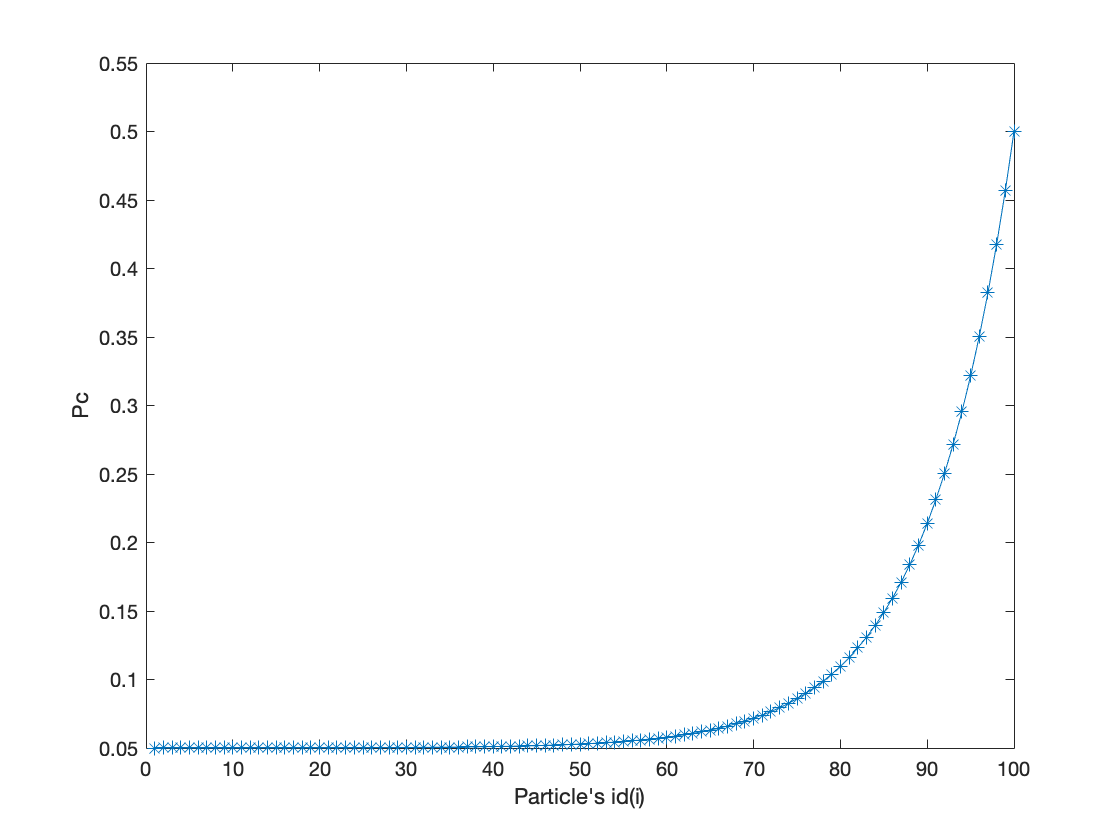
\includegraphics[scale=0.4]{./figure/Pc}
\caption{Each particle’s $Pc$ with a population size of 100.}
\label{fig:CLPSO_Pc}
\end{figure}

\par Compare the formula \ref{CLPSO_velocity} with the formula \ref{PSO_velocity_w_iter}, it is obviously that the `social experience' part is gone. And the `self-recognition' part is modified.
\newpage

\section{Parameter Tuning}
In this section, I use \textbf{Grid-search} for algorithmic parameter tuning.using 5 repetitions. And the test functions for tuning come from \cite{CEC-2017}. All results will be shown by mean and standard deviation.

For tuning, I chose \textit{Shifted and Rotated Zakharov Function, Shifted and Rotated Rosenbrock's Function, Shifted and Rotated Rastrigin's Function, Shifted and Rotated Expanded Scaffer’s F6 Function,Shifted and Rotated Lunacek Bi\_Rastrigin Function}. Shortly, the chosen functions are $f_1,f_3,f_4,f_5,f_6,f_7$(The function which index is 2 was been deleted). As shown in Table.\ref{tab:CEC-2017_test_function}

\begin{table}[h]
% \caption {a Part of the CEC’17 Test Functions} 
% \label{tab:CEC-2017_test_function} 
\begin{tabular}{|c|c|c|c|}
\hline
 & No. & Functions & $F_i^*=F_i(x^*)$ \\ \hline
\multirow{2}{*}{\begin{tabular}[c]{@{}c@{}}Unimodal\\ Functions\end{tabular}} & 1 & Shifted and Rotated Bent Cigar Function & 100 \\ \cline{2-4} 
 & 3 & Shifted and Rotated Zakharov Function & 300 \\ \hline
\multirow{4}{*}{\begin{tabular}[c]{@{}c@{}}Simple\\ Multimodal\\ Functions\end{tabular}} & 4 & Shifted and Rotated Rosenbrock’s Function & 400 \\ \cline{2-4} 
 & 5 & Shifted and Rotated Rastrigin’s Function & 500 \\ \cline{2-4} 
 & 6 & Shifted and Rotated Expanded Scaffer’s F6 Function & 600 \\ \cline{2-4} 
 & 7 & Shifted and Rotated Lunacek Bi\_Rastrigin Function & 700 \\ \hline
\multicolumn{4}{|c|}{Search Range: $[-100, 100]^D$} \\ \hline
\end{tabular}
\caption {Chosen functions for tuning from the CEC’17 Test Functions} 
\label{tab:CEC-2017_test_function} 
\end{table}

\subsection{PSO} As described in Section \textbf{1}, for PSO, there are 4 parameters that we can tune, which are $c_1, c_2, w_{max}, w_{min}$.  In fact, these two components also prevent the exploration and exploitation of the PSO algorithm. The $pbest$ pulls the particles to explore the optimal area within the whole searching range, while the $gbest$ pulls the particles to move to the existing optimal area. 
\subsubsection{Learning Factor}
\par When tuning learning factor $c_1, c_2$, I set the step length of Grid-search as $0.1$. And the search range for each parameter is $[1,2]$. In this way, we will get $10\times10$ combinations. In order to save space, the whole results table in .mat format can get on my Github homepage\footnote{https://github.com/bangjieding/course\_code.git/EE6227/Assignments/CEC2017-BoundContrained-master/codes/Matlab/tuning\_c1\_c2\_gbestval.mat}. The table only shows the best combination of $c_1$ and $c_2$ for each selected test function.

\par Table.\ref{tab:PSO_c_std} and Table.\ref{tab:PSO_c_mean} show the best performance on standard deviation and mean of each chosen function. From there two tables, we can observe that when $c_1 = \textbf{1.7}$ and $c_2 = \textbf{1.3}$ can combine the best learning factor.
\newpage
\begin{table}[!htb]
\centering
\begin{tabular}{|c|c|c|c|c|c|c|c|c|}
\hline
\multirow{2}{*}{line} & \multirow{2}{*}{$c_1$} & \multirow{2}{*}{$c_2$} & \multicolumn{2}{c|}{$f_3$} & \multicolumn{2}{c|}{$f_4$} & \multicolumn{2}{c|}{$f_5$}             \\ \cline{4-9} 
   &     &     & mean     & std\_dev       & mean   & std\_dev    & mean    & std\_dev    \\ \hline
1  & 1   & 1   & 300      & $\pm$0         & 400.17 & $\pm$0.0598 & 508.75  & $\pm$3.749  \\ \hline
22 & 1.1 & 2   & 3.00E+02 & $\pm$2.842E-14 & 400.24 & $\pm$0.023  & 507.36  & $\pm$4.371  \\ \hline
59 & 1.5 & 1.3 & 3.00E+02 & $\pm$2.842E-14 & 401.37 & $\pm$0.830  & 503.97  & $\pm$0      \\ \hline
4  & 1   & 1.3 & 3.00E+02 & $\pm$4.019E-14 & 400.21 & $\pm$0.06   & 505.96  & $\pm$2.900  \\ \hline
92 & 1.8 & 1.3 & 3.00E+02 & $\pm$4.019E-14 & 401.94 & $\pm$0.400  & 503.97  & $\pm$0.99   \\ \hline
   &     &     &          &                &        &             &         &             \\ \hline
\multirow{2}{*}{line} & \multirow{2}{*}{$c_1$} & \multirow{2}{*}{$c_2$} & \multicolumn{2}{c|}{$f_6$} & \multicolumn{2}{c|}{$f_7$} & \multicolumn{2}{c|}{\multirow{7}{*}{}} \\ \cline{4-7}
   &     &     & mean     & std\_dev       & mean   & std\_dev    & \multicolumn{2}{c|}{} \\ \cline{1-7}
1  & 1   & 1   & 600      & $\pm$2.542E-09 & 715.00 & $\pm$4.485  & \multicolumn{2}{c|}{} \\ \cline{1-7}
22 & 1.1 & 2   & 600      & $\pm$0         & 717.64 & $\pm$4.679  & \multicolumn{2}{c|}{} \\ \cline{1-7}
59 & 1.5 & 1.3 & 600      & $\pm$0         & 715.78 & $\pm$0.722  & \multicolumn{2}{c|}{} \\ \cline{1-7}
4  & 1   & 1.3 & 600      & $\pm$0         & 720.52 & $\pm$3.184  & \multicolumn{2}{c|}{} \\ \cline{1-7}
92 & 1.8 & 1.3 & 600      & $\pm$0         & 714.14 & $\pm$0.519  & \multicolumn{2}{c|}{} \\ \hline
\end{tabular}
\caption {The best performance on standard deviation of each chosen function.} 
\label{tab:PSO_c_std}
\end{table}

\begin{table}[!htb]
\centering
\begin{tabular}{|c|c|c|c|c|c|c|c|c|}
\hline
\multirow{2}{*}{line} & \multirow{2}{*}{$c_1$} & \multirow{2}{*}{$c_2$} & \multicolumn{2}{c|}{$f_3$} & \multicolumn{2}{c|}{$f_4$} & \multicolumn{2}{c|}{$f_5$} \\ \cline{4-9} 
   &     &     & mean & std\_dev      & mean   & std\_dev   & mean   & std\_dev   \\ \hline
1  & 1   & 1   & 300  & 0             & 400.17 & $\pm$0.059 & 508.75 & $\pm$3.749 \\ \hline
11 & 1   & 2   & 300  & $\pm$4.92E-14 & 400.12 & $\pm$0.084 & 508.35 & $\pm$6.07  \\ \hline
78 & 1.7 & 1   & 300  & $\pm$4.92E-14 & 401.2  & $\pm$1.072 & 502.38 & $\pm$1.13  \\ \hline
10 & 1   & 1.9 & 300  & $\pm$4.92E-14 & 400.22 & $\pm$0.134 & 505.96 & $\pm$2.814 \\ \hline
86 & 1.7 & 1.8 & 300  & $\pm$4.02E-14 & 401.45 & $\pm$0.866 & 505.57 & $\pm$1.664 \\ \hline
   &     &     &      &               &        &            &        &            \\ \hline
\multirow{2}{*}{line} & \multirow{2}{*}{$c_1$} & \multirow{2}{*}{$c_2$} & \multicolumn{2}{c|}{$f_6$} & \multicolumn{2}{c|}{$f_7$} &              &             \\ \cline{4-9} 
   &     &     & mean & std\_dev      & mean   & std\_dev   &        &            \\ \hline
1  & 1   & 1   & 600  & $\pm$2.54E-09 & 715.00 & $\pm$4.485 &        &            \\ \hline
11 & 1   & 2   & 600  & $\pm$0        & 718.17 & $\pm$4.48  &        &            \\ \hline
78 & 1.7 & 1   & 600  & $\pm$1.14E-13 & 716.15 & $\pm$2.633 &        &            \\ \hline
10 & 1   & 1.9 & 600  & $\pm$1.14E-13 & 716.69 & $\pm$4.06  &        &            \\ \hline
86 & 1.7 & 1.8 & 600  & $\pm$0        & 712.14 & $\pm$4.589 &        &            \\ \hline
\end{tabular}
\caption {The best performance on mean of each chosen function.}
\label{tab:PSO_c_mean}
\end{table}


\subsection{Inertia Weight}
\par As mentioned in section \textbf{1}, the inertial weight is introduced by Shi\cite{shi}, and the larger the w, the stronger global search ability, and the weaker local search ability, with the smaller the value, the weaker global search ability, and the stronger local search ability. 
\par When tuning inertia weight $w$, I set the step length of one-dimension Grid-search as 0.1. Also, $the search range \in[0.1,1.0]$. And compute $w_i$ according to the formula \ref{PSO_velocity_w_w}. Also, the whole table of tuning $w_{max}$ and $w_{min}$ can be seen on my Github homepage\footnote{https://github.com/bangjieding/course\_code.git/EE6227/Assignments/CEC2017-BoundContrained-master/codes/Matlab/tuning\_wmax\_wmin.mat}.
\begin{table}[!h]
\begin{tabular}{|c|c|c|c|c|c|c|c|c|}
\hline
\multirow{2}{*}{line} &
  \multirow{2}{*}{$w_{max}$} &
  \multirow{2}{*}{$w_{min}$} &
  \multicolumn{2}{c|}{$f_3$} &
  \multicolumn{2}{c|}{$f_4$} &
  \multicolumn{2}{c|}{$f_5$} \\ \cline{4-9} 
   &     &     & mean   & std\_dev      & mean   & std\_dev    & mean     & std\_dev      \\ \hline
7  & 0.5 & 0.1 & 300    & $\pm$5.68E-14 & 411.99 & $\pm$15.353 & 519.56   & $\pm$11.6598  \\ \hline
16 & 0.7 & 0.1 & 300    & $\pm$4.02E-14 & 400.30 & $\pm$0.224  & 505.63   & $\pm$2.07116  \\ \hline
31 & 0.9 & 0.3 & 300    & $\pm$0        & 401.10 & $\pm$0.6438 & 503.31   & $\pm$1.1488   \\ \hline
39 & 1   & 0.3 & 300    & $\pm$4.02E-14 & 401.48 & $\pm$1.0390 & 505.6    & $\pm$1.1488   \\ \hline
26 & 0.8 & 0.5 & 300    & $\pm$0        & 401.62 & $\pm$0.516  & 506.3014 & $\pm$0.5744   \\ \hline
8  & 0.5 & 0.2 & 300    & $\pm$0        & 406.36 & $\pm$0.2831 & 517.245  & $\pm$3.039    \\ \hline
36 & 0.9 & 0.8 & 300    & $\pm$0        & 402.88 & $\pm$0.0568 & 506.301  & $\pm$1.51982  \\ \hline
43 & 1   & 0.7 & 300    & $\pm$0        & 401.80 & $\pm$0.4233 & 504.97   & $\pm$6.96E-14 \\ \hline
19 & 0.7 & 0.4 & 300    & $\pm$0        & 401.31 & $\pm$0.7817 & 507.62   & $\pm$5.00784  \\ \hline
41 & 1   & 0.5 & 300    & $\pm$4.02E-14 & 401.87 & $\pm$0.4354 & 503.97   & $\pm$1.98991  \\ \hline
\multicolumn{9}{|c|}{}                                                                    \\ \hline
\multirow{2}{*}{line} &
  \multirow{2}{*}{$w_{max}$} &
  \multirow{2}{*}{$w_{min}$} &
  \multicolumn{2}{c|}{$f_6$} &
  \multicolumn{2}{c|}{$f_7$} &
  \multicolumn{2}{c|}{\multirow{12}{*}{}} \\ \cline{4-7}
   &     &     & mean   & std\_dev      & mean   & std\_dev    & \multicolumn{2}{c|}{}    \\ \cline{1-7}
7  & 0.5 & 0.1 & 600.62 & $\pm$0.866    & 722.96 & $\pm$4.8599 & \multicolumn{2}{c|}{}    \\ \cline{1-7}
16 & 0.7 & 0.1 & 600    & $\pm$0.0002   & 719.07 & $\pm$2.4656 & \multicolumn{2}{c|}{}    \\ \cline{1-7}
31 & 0.9 & 0.3 & 600    & $\pm$0        & 714.5  & $\pm$2.7196 & \multicolumn{2}{c|}{}    \\ \cline{1-7}
39 & 1   & 0.3 & 600    & $\pm$1.14E-13 & 716.01 & $\pm$1.6854 & \multicolumn{2}{c|}{}    \\ \cline{1-7}
26 & 0.8 & 0.5 & 600    & $\pm$0        & 710.38 & $\pm$6.9813 & \multicolumn{2}{c|}{}    \\ \cline{1-7}
8  & 0.5 & 0.2 & 600.50 & $\pm$0.8569   & 725.06 & $\pm$7.4967 & \multicolumn{2}{c|}{}    \\ \cline{1-7}
36 & 0.9 & 0.8 & 600    & $\pm$0        & 716.08 & $\pm$2.2588 & \multicolumn{2}{c|}{}    \\ \cline{1-7}
43 & 1   & 0.7 & 600    & $\pm$0        & 716.69 & $\pm$1.3589 & \multicolumn{2}{c|}{}    \\ \cline{1-7}
19 & 0.7 & 0.4 & 600    & $\pm$0        & 717.65 & $\pm$1.6689 & \multicolumn{2}{c|}{}    \\ \cline{1-7}
41 & 1   & 0.5 & 600    & $\pm$0        & 714.05 & $\pm$0.6832 & \multicolumn{2}{c|}{}    \\ \hline
\end{tabular}
\caption {The best performance on mean and standard deviation of each chosen function.}
\label{tab:PSO_w}
\end{table}
\par From Table. \ref{tab:PSO_w}, we can get that the best combination of the performance of $w_{max}$ and $w_{min}$ is $w_{max}=\textbf{0.9}$ and $w_{min}=\textbf{0.3}$. And according to the formula \ref{PSO_velocity_w_w}, the expression now comes to as following:

\begin{equation}
w_{iter} = 0.9 - \dfrac{0.9 - 0.3}{iter_{max}}\times iter 
\label{PSO_velocity_w_w_numerical}
\end{equation}
Where the $iter_{max}$ is the maximum times of iterations, $iter$ represents the $iter^{th}$ iteration.







\newpage
\begin{thebibliography}{99}
\bibitem{PSO_1}
R. C. Eberhart and J. Kennedy, “A new optimizer using particle swarm theory,” in Proc. 6th Int. Symp. Micromachine Human Sci., Nagoya, Japan, 1995, pp. 39–43.

\bibitem{PSO_2}
J. Kennedy and R. C. Eberhart, “Particle swarm optimization,” in Proc. IEEE Int. Conf. Neural Networks, 1995, pp. 1942–1948.

\bibitem{shi}
Y. Shi and R. C. Eberhart, “A modified particle swarm optimizer,” in Proc. IEEE Congr. Evol. Comput., 1998, pp. 69–73.

\bibitem{J.Liang}
J.J. Liang, A.K. Qin, P.N. Suganthan, S. Baskar, “Comprehensive learning particle swarm optimizer for global optimization of multimodal functions,” IEEE Trans. Evol. Comput., 2006, pp. 281–295.

\bibitem{CEC-2017}
N. H. Awad, M. Z. Ali, J. J. Liang, B. Y. Qu and P. N. Suganthan, “Problem Definitions and Evaluation Criteria for the CEC 2017 Special Session and Competition on Single Objective Bound Constrained Real-Parameter Numerical Optimization,”  Technical Report, Nanyang Technological University, Singapore, November 2016.

\end{thebibliography}


\end{document}
